\chapter{2020-04-21}
%\begin{document}

%    \maketitle
    
%    \begin{abstract}
        
%    \end{abstract}
    
%    \tableofcontents
 %   \thispagestyle{empty}
  %  \newpage
   % \setcounter{page}{1}
\section{Model Architecture}
\begin{figure}[!ht]
    \centering
    %\begin{adjustbox}{width=\textwidth}
   % \begin{adjustbox}{max width=\textwidth,height=8cm}
    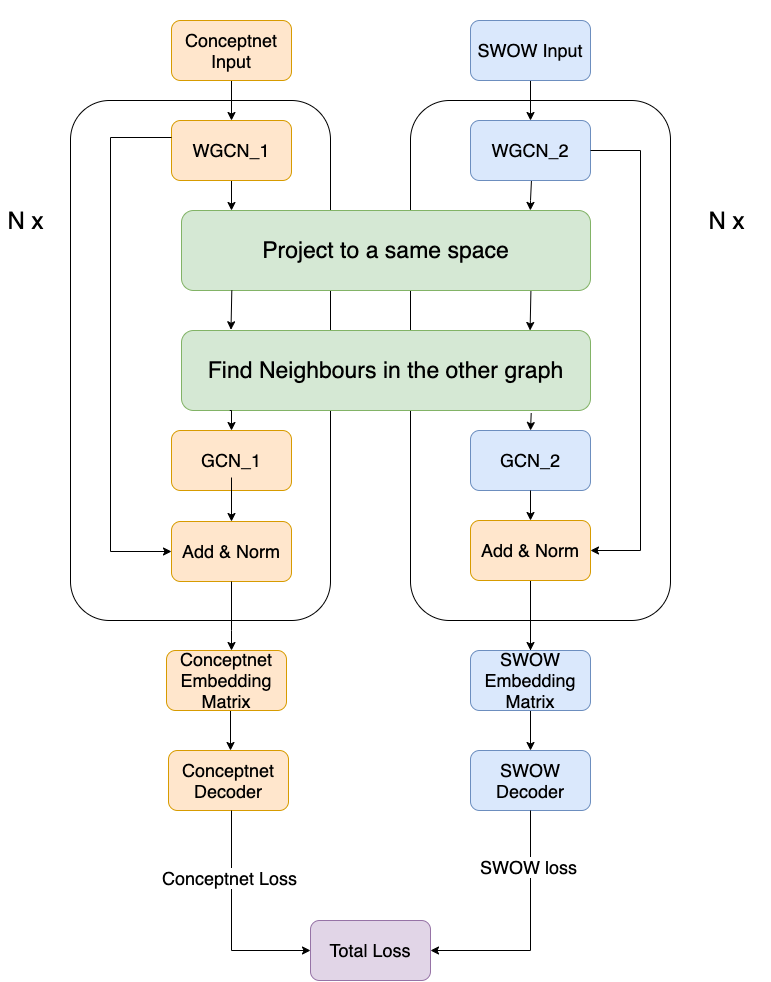
\includegraphics[scale=0.45]{images/conceptnet-swow.png}
   % \caption{Caption}
     \label{fig:concept-swow-model-architecture}
     %\end{adjustbox}
\end{figure}

In previous methods, the neighbours of a node in a graph are static or fixed, and will not updated during the whole training process. The core view of this idea is to update the neighbours of a node in the training process. In this way, we can compute the neighbours of a the node and thus gain a another embedding for this node. Then, for each node, we can combine the two embeddings with different weight to gain a new embedding.  For the sources of the neighbours, there can be two options, from the its own graph and another graph. If it is from its own graph, then it can be seen as the "self-attention" in Transformer. 
If it's from another graph, it can introduce more external knowledge. 
One thing needs to be noted is that we can only obtain the neighbour nodes, the edge label (relation type) information cannot be obtained. So the GCN for initial graph and updated graph will be a little bit different. Take the latter option for example, the process can be formulated with the following equations: \\

\noindent Notations: \\ 
C: the initial ConceptNet graph  (with initialized node embedding matrix, relation types, each node has initial neighbours)\\
S: the initial SWOW graph.  (similar as ConceptNet)
\\$C_n$: updated Concept graph with neighbours from SWOW (with nodes in original ConceptNet and also their embeddings. Each node has a set of neighbours, whose embeddings come from SWOW, no relation types) \\ 
$S_n$: updated SWOW graph with neighbours from ConceptNet. (similar to $C_n$)

\begin{align}
\mathbf{E_{c} } & = WGCN(C),  & \mathbf{E_{s}}  & = WGCN(S) \label{formula:gcn}\\
 \mathbf{E_{c}^m} & = f_m(\mathbf{E_c}), &  \mathbf{E_{s}^m} & =f_m(\mathbf{E_s}) \label{formula:prjection} \\
C_n  &= g(\mathbf{E_{c}^m}, \mathbf{E_{s}^m}),  & S_n  & = g(\mathbf{E_{s}^m}, \mathbf{E_{c}^m})   \label{formula:find_neighbours} \\
    \mathbf{E_c^{\prime}}& = GCN(C_n),   & \mathbf{E_s^{\prime}} & =GCN(S_n) \label{formula:gcn2} \\
    E_c^o  &= f_l(\mathbf{E_c } + \mathbf{E_c^{\prime}}), & E_s^o & = f_l(\mathbf{E_s } + \mathbf{E_s^{\prime}}),  \label{formula:layrnorm}
\end{align}
Equation~\ref{formula:prjection} uses function $f_m$ to project the two embedding matrices into a same space\\
Equation~\ref{formula:find_neighbours}  finds the neighbours in in each other's graph.\\
Equation~\ref{formula:gcn2} passes the new graph (neighbours are from another graph) to another gcn.\\
Equation~\ref{formula:layrnorm} adds the two embedding matrices from two gcn layer and performs a layernorm on them.


The above five equations will be wrapped as a whole and repeated many times. 

%\printbibliography


%\section{To do list}
%

%\end{document}

